\documentclass{exam}
\usepackage[utf8]{inputenc}
\usepackage{lmodern}
\usepackage{microtype}

% \usepackage[parfill]{parskip}
\usepackage[dvipsnames]{xcolor}
\usepackage{amsmath}
\usepackage{amsfonts}
\usepackage{amsthm}
\usepackage{siunitx}
\DeclareSIUnit\year{yr}
\DeclareSIUnit\foot{ft}
\DeclareSIUnit\litre{\liter}

\usepackage{skull}

\usepackage{pgfplots}
\usepgfplotslibrary{polar}
\pgfplotsset{compat=1.11}
\usepgfplotslibrary{statistics}
\usepackage{graphicx}
\usepackage{sidecap}
\sidecaptionvpos{figure}{c}
\usepackage{float}
\usepackage{gensymb}
\usepackage{tkz-euclide}
\usetkzobj{all}
\usepackage{commath}
\usepackage{hyperref}
\usepackage{enumitem}
\usepackage{wasysym}
\usepackage{multicol}
\usepackage{mathtools}
\usepackage{tcolorbox}
\usepackage{tabularx}
\usepackage[version=4]{mhchem}
\usepackage{changepage}
\usepackage{listings}
\lstset{basicstyle=\ttfamily\linespread{0.8}\small}

\renewcommand*{\thefootnote}{\fnsymbol{footnote}}

\newtheorem*{thm}{Theorem}
\newtheorem*{iden}{Identity}
\newtheorem*{lemma}{Lemma}
\newtheorem{obs}{Observation}
\theoremstyle{definition}
\newtheorem*{defn}{Definition}
\newtheorem*{ex}{Example}
\newtheorem{con}{Construction}
\newtheorem*{alg}{Algorithm}

\newtheoremstyle{break}
  {\topsep}{\topsep}%
  {\itshape}{}%
  {\bfseries}{}%
  {\newline}{}%
\theoremstyle{break}
\newtheorem*{bthm}{Theorem}

% russian integral
\usepackage{scalerel}
\DeclareMathOperator*{\rint}{\scalerel*{\rotatebox{17}{$\!\int\!$}}{\int}}

% \DeclareMathOperator*{\rint}{\int}

\pgfplotsset{vasymptote/.style={
    before end axis/.append code={
        \draw[densely dashed] ({rel axis cs:0,0} -| {axis cs:#1,0})
        -- ({rel axis cs:0,1} -| {axis cs:#1,0});
    }
}}

% \pointsinrightmargin
\boxedpoints
\pointname{}

\newcommand{\questioA}{\question[\texttt{\textbf{\color{Cerulean} A}}]}
\newcommand{\questioM}{\question[\texttt{\textbf{\color{PineGreen} M}}]}
\newcommand{\questioE}{\question[\texttt{\textbf{\color{WildStrawberry} E}}]}
\newcommand{\questioS}{\question[\texttt{\textbf{\color{Goldenrod} S}}]}
\newcommand{\questioO}{\question[\texttt{\textbf{\color{BurntOrange} O}}]}

\newcommand{\parA}{\part[\texttt{\textbf{\color{Cerulean} A}}]}
\newcommand{\parM}{\part[\texttt{\textbf{\color{PineGreen} M}}]}
\newcommand{\parE}{\part[\texttt{\textbf{\color{WildStrawberry} E}}]}
\newcommand{\parS}{\part[\texttt{\textbf{\color{Goldenrod} S}}]}
\newcommand{\parO}{\part[\texttt{\textbf{\color{BurntOrange} O}}]}

\newcommand{\subparA}{\subpart[\texttt{\textbf{\color{Cerulean} A}}]}
\newcommand{\subparM}{\subpart[\texttt{\textbf{\color{PineGreen} M}}]}
\newcommand{\subparE}{\subpart[\texttt{\textbf{\color{WildStrawberry} E}}]}
\newcommand{\subparS}{\subpart[\texttt{\textbf{\color{Goldenrod} S}}]}
\newcommand{\subparO}{\subpart[\texttt{\textbf{\color{BurntOrange} O}}]}

\newcommand{\mainHeader}[2]{\section*{NCEA Level 2 Mathematics\\#1. #2}}
\newcommand{\mainHeaderHw}[2]{\section*{NCEA Level 2 Mathematics (Homework)\\#1. #2}}
\newcommand{\seealso}[1]{\begin{center}\emph{See also #1.}\end{center}}
\newcommand{\drills}[1]{\begin{center}\emph{Drill problems: #1.}\end{center}}
\newcommand{\basedon}[1]{\begin{center}\emph{Notes largely based on #1.}\end{center}}

\usepackage[normalem]{ulem}
\usepackage{venndiagram}
\begin{document}

\pgfmathdeclarefunction{gauss}{2}{%
  \pgfmathparse{1/(#2*sqrt(2*pi))*exp(-((x-#1)^2)/(2*#2^2))}%
}


\mainHeader{22}{Probability Distributions}

We have now looked at `discrete' probabilities: probabilities relating to experiments
in which there are a finite number of outcomes. There are six outcomes when a die
is rolled, there are two possibilities for flipping a coin, and so on.

Now, we will look briefly at `continuous' probabilities. These arise when we perform
experiments involving real-world measurements: if we measure the heights of a thousand
people, each one will have a slightly different reading.

Our question then becomes `what is the probability that our reading falls between $ x_0 $
and $ x_1 $', rather than `what is the probability of a reading $ x $'.

It turns out that most `natural' experiments produce probabilities fitting what is
known as a \emph{normal curve}, or \emph{standard distribution}. Such a curve is
determined by two numbers: a standard deviation $ \sigma $ that determines the spread
of the curve (the width), and a mean value $ \mu $ which tells us where the peak is.

\begin{center}
  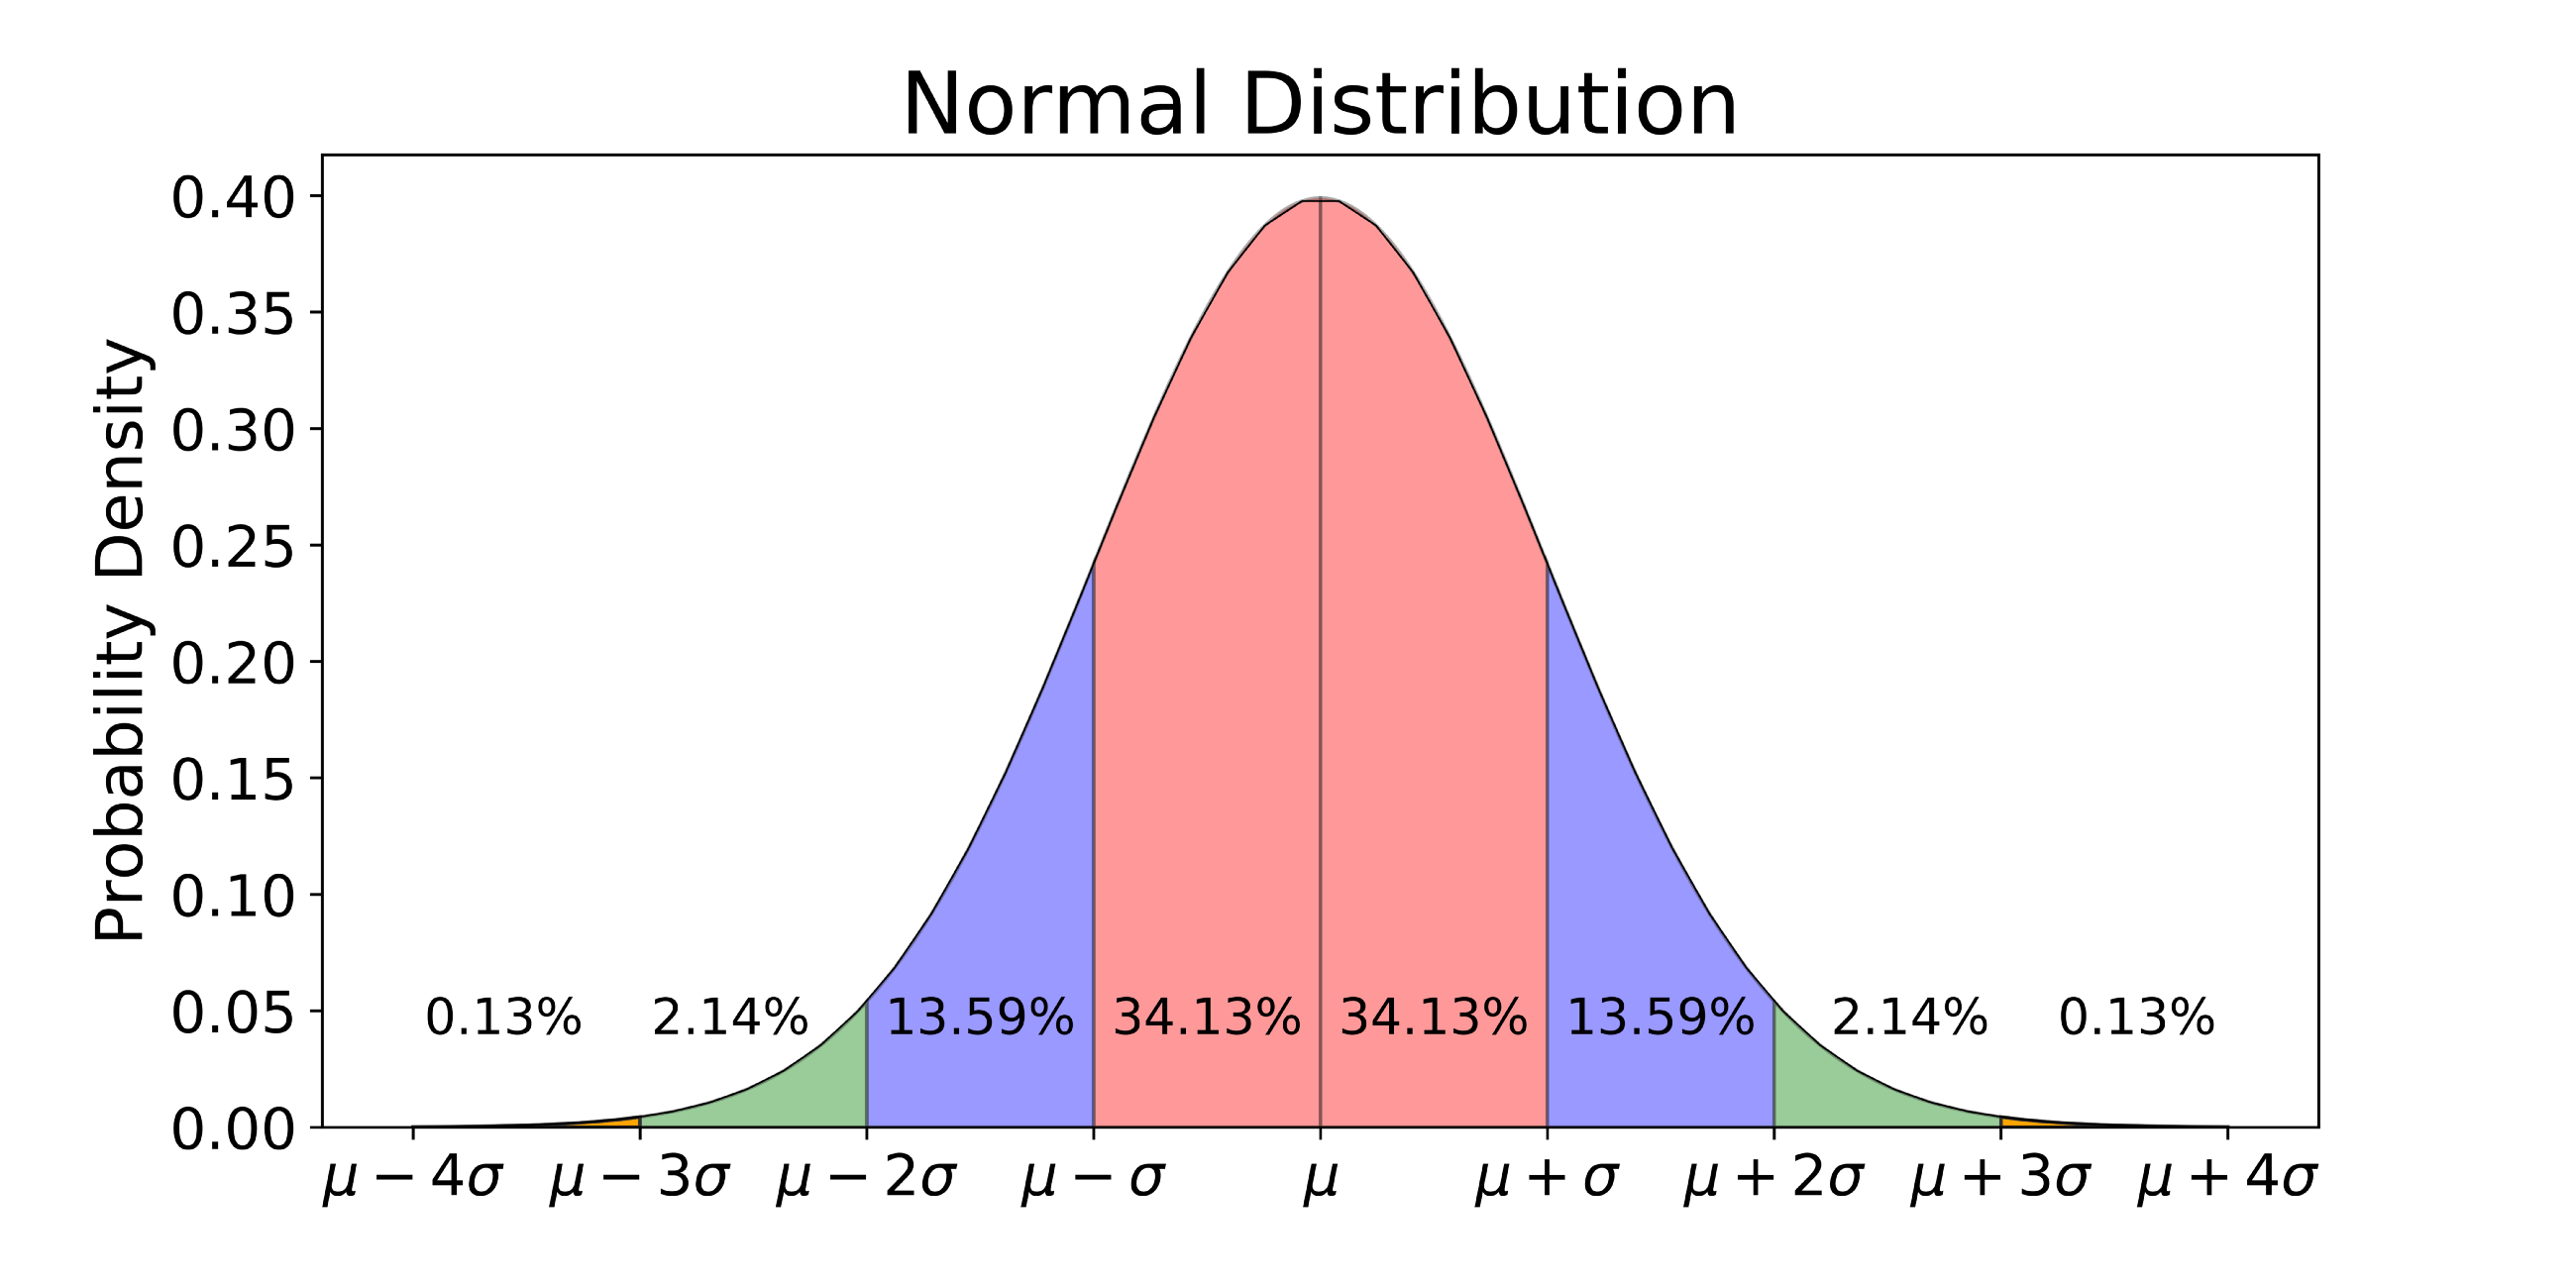
\includegraphics[width=\textwidth]{norml}
\end{center}

The $ x$-axis represents possible measurement values. The probability of a value lying
between the measurements $ x_0 $ and $ x_1 $ is the area underneath the curve between
the lines $ x = x_0 $ and $ x = x_1 $. The height of the curve at any given point has no
meaning, only the area.

The \emph{standardised} normal curve has mean $ \mu = 0 $ and standard deviation $ \sigma = 1 $.
If our random variable is $ X $, and we want to find the probability it lies between $ x_0 $ and $ x_1 $
given some mean $ \mu $ and standard deviation $ \sigma $, then we can transform our problem
to one involving a random variable $ Z $ and the standardised curve: our probability will
be the area under the standardised curve between $ z_0 = (x_0 - \mu)/\sigma $ and $ z_1 = (x_1 - \mu)/\sigma $.
This can be summarised by writing
\begin{displaymath}
  Z = \frac{X - \mu}{\sigma}.
\end{displaymath}

The table given in the NCEA L2 external formula sheet gives the area under the standardised curve between 0 and $ z $;
it is reproduced over the page.

\paragraph{Note.} The formula for the normal distribution curve with mean $ \mu $ and standard deviation $ \sigma $ is
\begin{displaymath}
  y = \frac{1}{\sqrt{2\pi \sigma^2}} \exp\left(-\frac{(x - \mu)^2}{2\sigma^2}\right).
\end{displaymath}

\clearpage
\begin{center}
  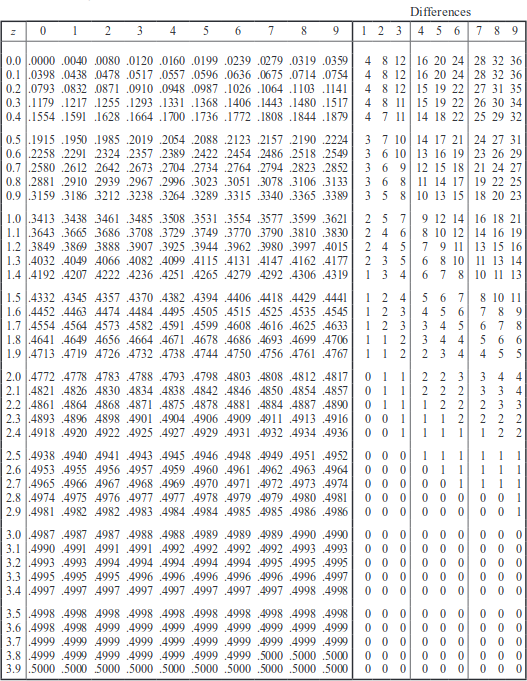
\includegraphics[height=0.8\textheight]{distributiontable}
\end{center}
\clearpage

\subsection*{Questions}
\begin{questions}
  \question A manufacturing company finds the life of a battery for a product to be normally distributed, with mean 4 years and standard
            deviation 1 year.
    \begin{parts}
      \part Given a randomly chosen battery, what is the chance it lasts between three and five years?
      \part Given 10\,000 batteries, how many should be expected to have an abnormally short lifespan (less than two years)?
      \part What is the minimum length of life for the longest-lived 10\%?
    \end{parts}
  \question In the 2017 Census at School, 866 Y12 students answered the following question: `What is your height (nearest cm), without shoes on?'.
            The mean of this sample was \SI{170.6}{\centi\metre}, and the standard deviation was \SI{9.476}{\centi\metre}.
    \begin{parts}
      \part Draw a standard deviation fitting these parameters.
      \part What is the probability that a random individual from this sample has a height:
        \begin{subparts}
          \subpart Between 160 and 180 centimetres?
          \subpart Less than 150 centimetres?
        \end{subparts}
      \part What is the minimum height of the tallest 10\% of people? (In other words,
            which height $ x $ is such that there is a 0.1 probability that a sampled
            individual has a height greater than $ x $?)
      \part A histogram for the responses is given below.
            \begin{center}
              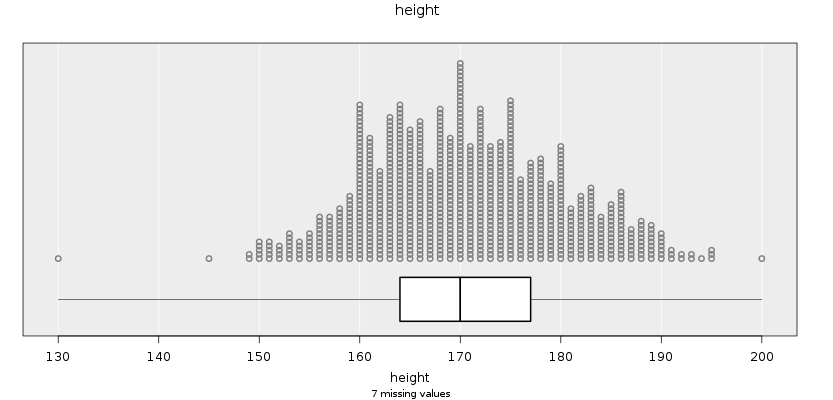
\includegraphics[width=0.8\textwidth]{heightdistribution}
            \end{center}
            Compare the normal distribution and the histogram that resulted from the sample
            results.

            In your answer you should consider the shape, centre, and spread of both distributions,
            and should provide numerical evidence where appropriate.
      \part In a given school, 10\% of year 12 students were taller than \SI{175.0}{\centi\metre},
            and the mean height of the students was \SI{167.2}{\centi\metre}.
        \begin{subparts}
          \subpart What is the standard deviation of this smaller sample of students?
          \subpart In this school, what was the maximum height of the shortest 20\% of students?
          \subpart What is the probability that, given two randomly selected Y12 students at this school,
                   both have heights greater than \SI{180}{\centi\metre}? (You may assume that all
                   heights are independent --- e.g. there are no identical twins.)
        \end{subparts}
    \end{parts}
  \question The grades of students in a certain course have a mean of 71.04\% and a standard deviation
            of 21.168 percentage points.
    \begin{parts}
      \part Assuming the grades match a standard distribution, what is the probability that a randomly
            chosen student passed (had a grade of greater than 50\%)?
      \part The following histogram depicts the actual grade distribution.
            \begin{center}
              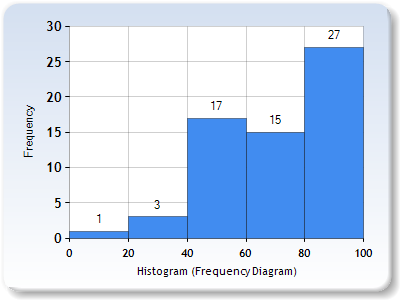
\includegraphics[width=0.4\textwidth]{distributiontable2}
            \end{center}
            Discuss whether a normal distribution would actually be a good fit for this data.
      \part Using the histogram, compute the probability that a randomly chosen student passed.
    \end{parts}
\end{questions}

\end{document}

